\documentclass{article}
\usepackage{booktabs}
\usepackage{graphicx}
\usepackage{amsmath}
\usepackage[a4paper, total={7in, 11in}]{geometry}
\usepackage[toc,page]{appendix}
\usepackage{listings} % Listing package to add appendix
\usepackage{xcolor}   % Custom colors
\usepackage{graphicx}  % Required to include images
\usepackage{hyperref}% to put links
\usepackage{float} %to place correctly pictures


\hypersetup{
    colorlinks=true,
    linkcolor=blue,
    urlcolor=blue,
    citecolor=red,
    linktoc=all,    % Links entire section titles in the ToC
    linkcolor=black % Sets ToC links to black; other links remain as specified
}

% Defining colors for the python section
\definecolor{codegreen}{rgb}{0,0.6,0}
\definecolor{codeblue}{rgb}{0,0,0.8}
\definecolor{codepurple}{rgb}{0.58,0,0.82}
\definecolor{codebackground}{rgb}{0.95,0.95,0.92}
\begin{document}

\title{Mid term Exam for Financial Econometrics with Python}
\author{PRAT Paul; GAVINI Charles; FOURNIER Justin; BLANC Mathieu}
\date{\today}

\maketitle %showcase the title in the top of the page with the informations upper

\tableofcontents %creating a table of contens

%first, introduction
\section{Introduction}
For the midterm assignment, we composed a group of 4 with Gavini Charles; Fournier Justin; Prat Paul and Blanc Mathieu. 
This document contains all the results of our assignment, including tables, figures, and calculations. 
It is composed by \arabic{section} parts, first, importing the good python libraries,
then initialising variables to separate the differents datas (daily, monthly, ..., returns, logreturns,...)


\section{Preliminary}
%Instructions


%At the beginning of your answer to Question 1, indicate clearly:
%- the name and the exact ticker of stock or index you are considering,
%- the length of your sample (number of days, months, years),
%- the initial and final dates of your sample, and
%- the stock market and country in which the stock you selected is traded, or to which the stock index you selected refers to.
%Using the time series you downloaded in PRELIMINARY STEP 1, compute the log-returns at daily, 
%monthly, and annual frequencies and present a table of summary statistics of these three series of returns. 
%The table should be similar to the one appearing in slide n. 91 of the set of slides titled 
%``Lecture 1: Financial Returns: Description and Stylized Facts’’.
\subsection{AMAZON}

The chosen stock is Amazon, because it is higly related in the current actuality. We are very interested in a major company such as Amazon, which has grown significantly over time.
The ticker from yahoo finance is " \textbf{\textit{AMZN}} " on the Nasdaq stock exchange \href{https://finance.yahoo.com/quote/AMZN/.}{AMAZON on Yahoo Finance}
First, importing the Amazon stock with yfinance, then display the pandas table.
We will import 25 years, 8 months and 25 days of data (from 1999-01-21 to 2024-10-16).

\subsection{Data Table}
The data printed here, is the preview of the Amazon stock extraction from yahoo fiannce:
% LaTeX table from 'table.tex'
\begin{table}[h!]
    \centering
    \begin{tabular}{lrrrrrr}
\toprule
{} &      Open &      High &       Low &     Close &  Adj Close &     Volume \\
Date       &           &           &           &           &            &            \\
\midrule
1999-09-16 &  0.051563 &  0.052083 &  0.050260 &  0.050911 &   0.046693 &  158112000 \\
1999-09-17 &  0.050586 &  0.051042 &  0.048958 &  0.050781 &   0.046574 &  171648000 \\
1999-09-20 &  0.049870 &  0.050521 &  0.048958 &  0.048958 &   0.044902 &  229104000 \\
1999-09-21 &  0.047917 &  0.048177 &  0.043620 &  0.044271 &   0.040603 &  737328000 \\
1999-09-22 &  0.044271 &  0.045573 &  0.041667 &  0.045313 &   0.041559 &  375984000 \\
\bottomrule
\end{tabular}
  
    \caption{Preview of Amazon Stock Data from Yahoo Finance}
    \label{tab:amazon_stock_preview}
\end{table}



\subsection{Checking the 25 Years range condition}

We have to check that the data is correctly displayed over a 25years range, hopefully, 
the introduction from Amazon is from january 1999, so it we should be able to find a 25 year range
of data of the Amazon stock. To check that we can compute a python code to count the gaps and visualize 
the dates of gaps in order to see for any huge gap that would be problematic for analyzing data.

\begin{figure}[H]
    \centering
    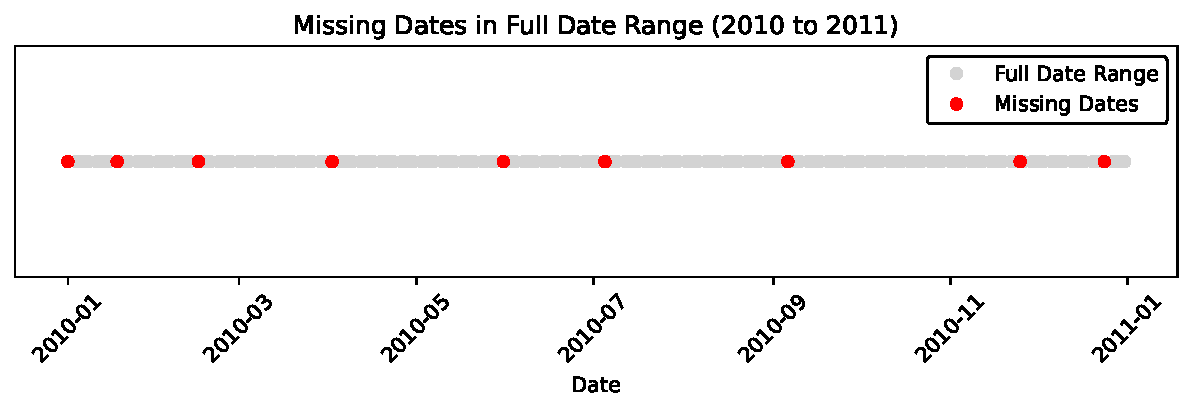
\includegraphics[width=\textwidth]{Img/MissingDates(2010_to_2011).pdf}
    \caption{Missing Dates in Full Date Range (2010 to 2011)}
    \label{fig:missing_dates}
\end{figure}

We count only 9 days without data over the 25-year range. Thus, the full data contains at least 25 years of values

\section{First Results}

\subsection{Prices Evolutions}

Then, ploting the prices evolution:

\begin{figure}[H]
    \centering
    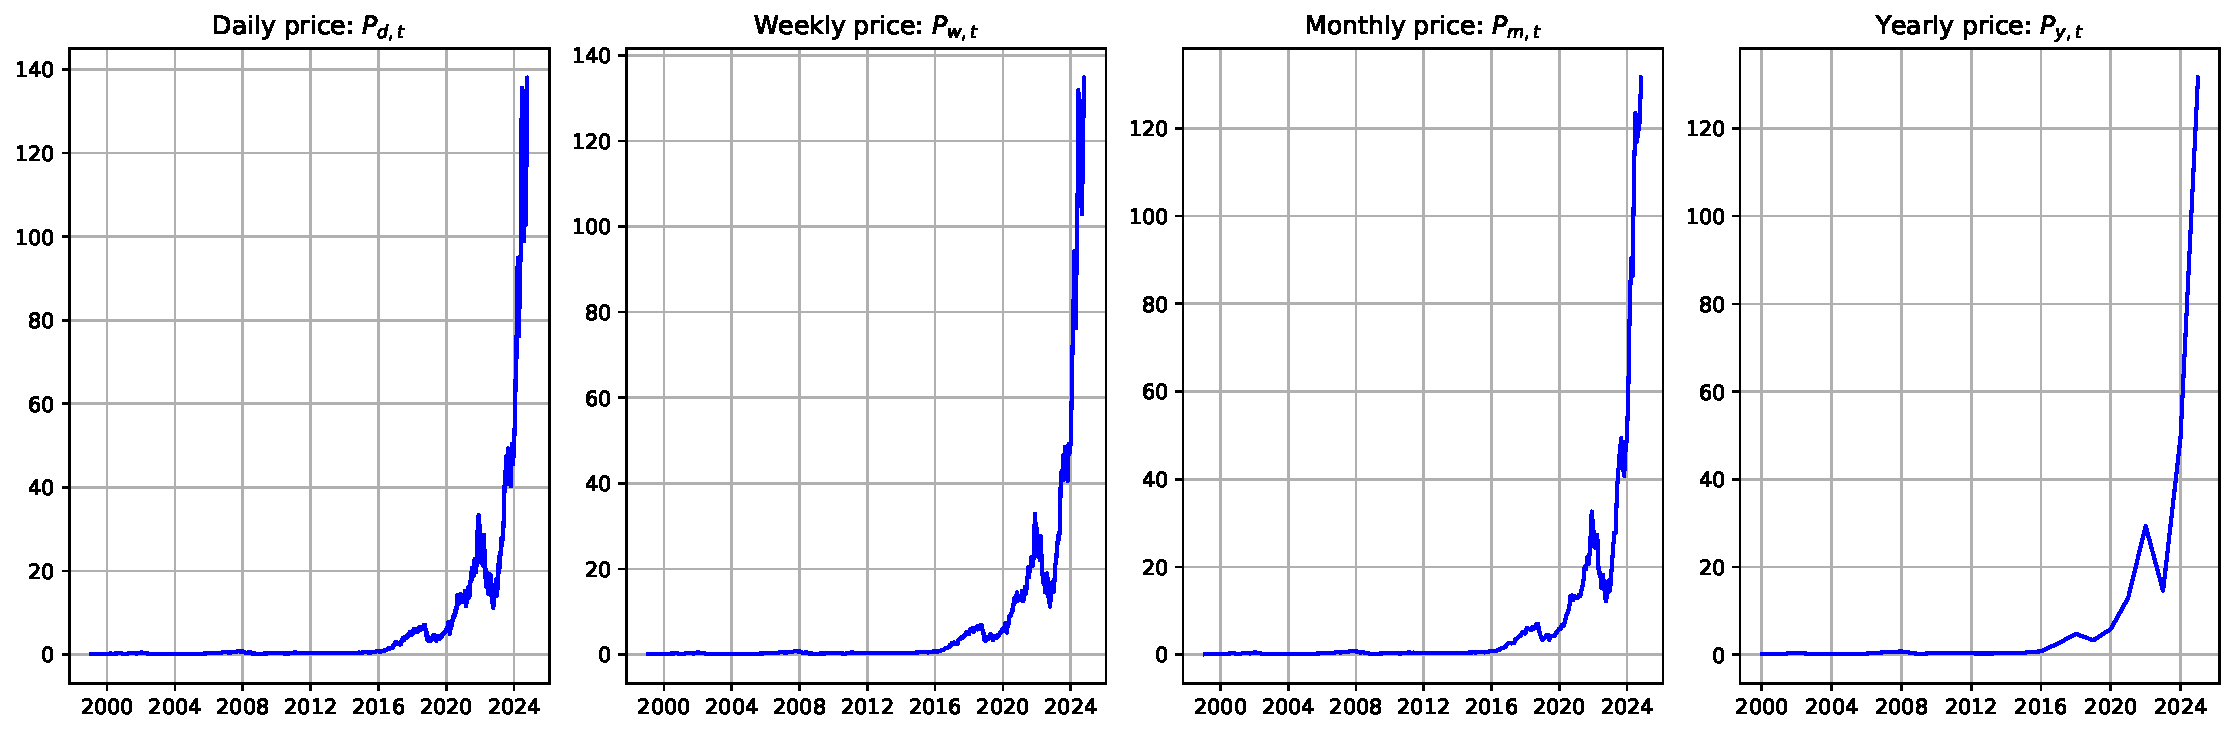
\includegraphics[width=\textwidth]{Img/prices_time.pdf}
    \caption{Prices over time by frequency}
    \label{fig:prices_time}
\end{figure}

\subsection{Calculating Returns}

\begin{figure}[H]
    \centering
    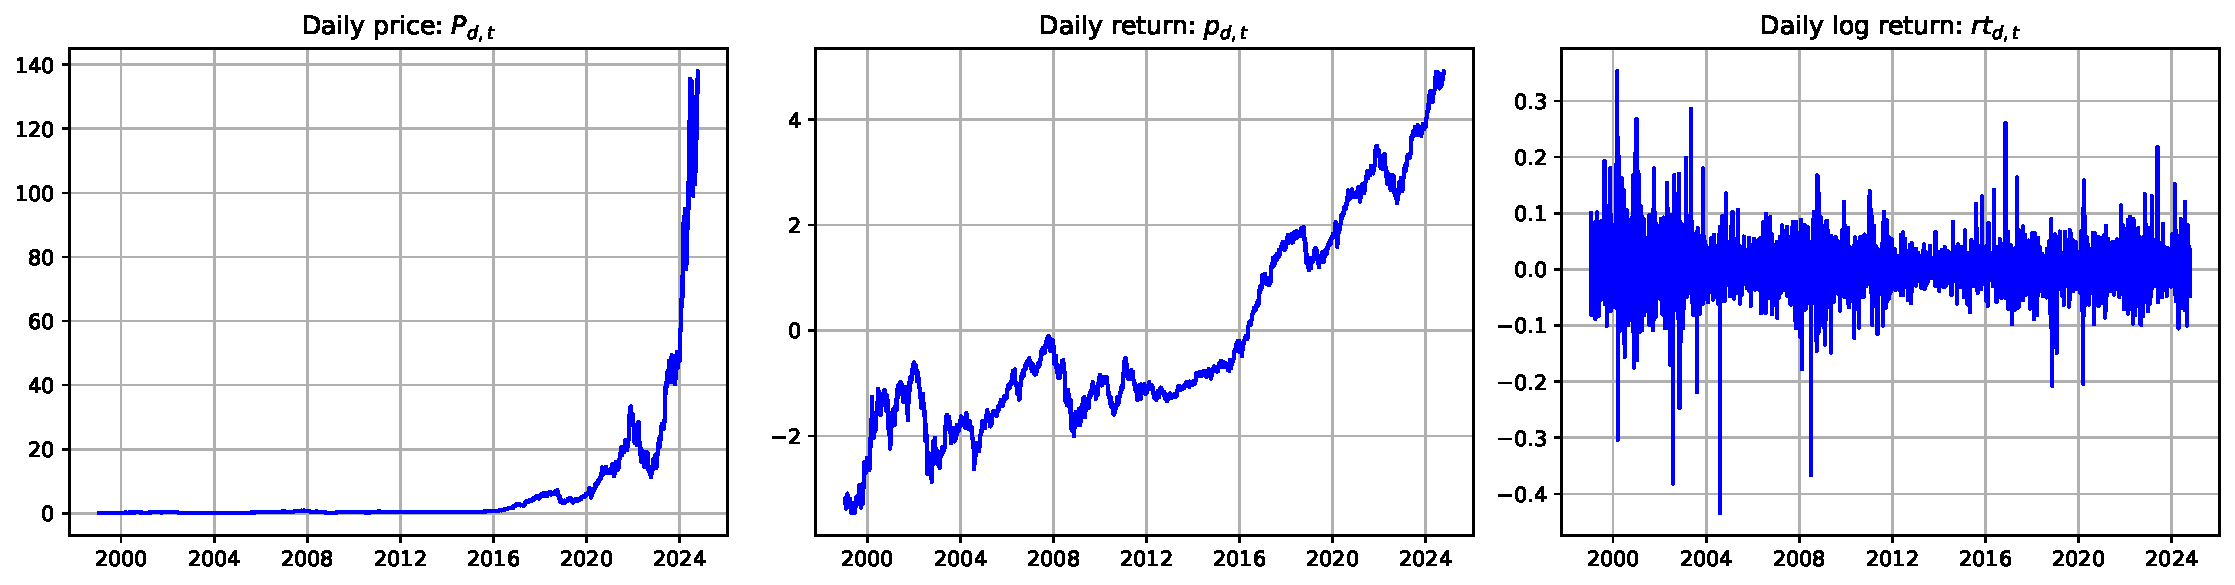
\includegraphics[width=\textwidth]{Img/log_returns.pdf}
    \caption{Prices, returns and log returns}
    \label{fig:log_returns}
\end{figure}

\subsection{Squared Returns}

\begin{figure}[H]
    \centering
    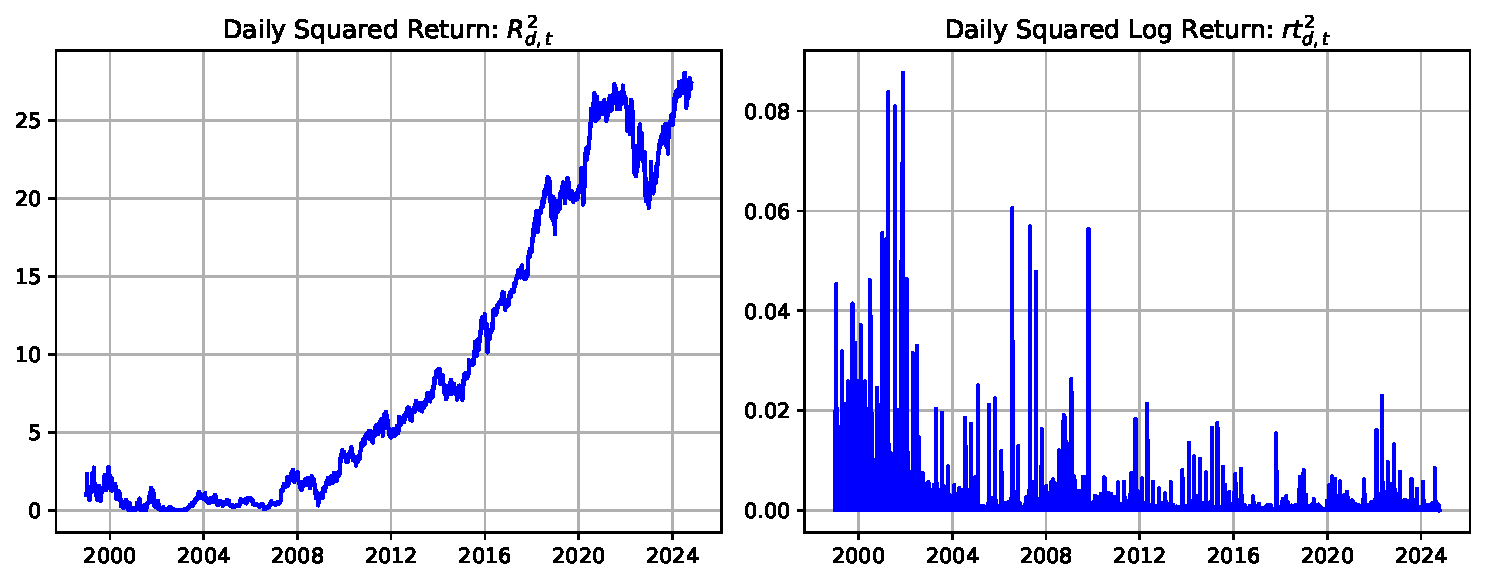
\includegraphics[width=\textwidth]{Img/squared_log_returns.pdf}
    \caption{Squared daily returns and daily log returns}
    \label{fig:squared_logreturns}
\end{figure}

\section{Amazon and the 8 Stylized Facts}
\subsection{Prices are non-stationary}

The first feature that will highlight non-stationarity of the prices is the comparison of \( p(t) \) vs \( p(t-1) \).

\begin{figure}[H]
    \centering
    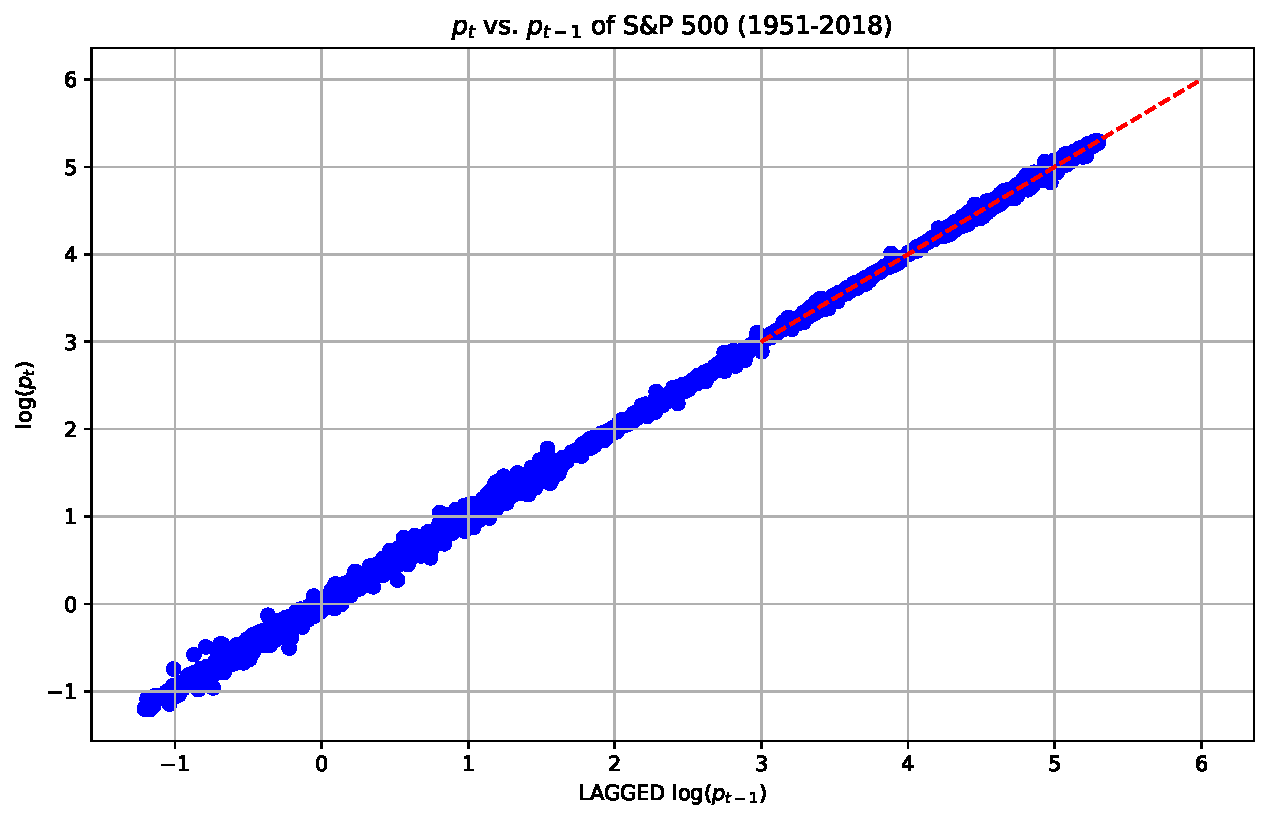
\includegraphics[width=0.8\textwidth]{Img/LogptVSLogpt-1.pdf}
    \caption{Comparison of \( \log(p_t) \) vs \( \log(p_{t-1}) \)}
    \label{fig:LogptVSLogpt-1}
\end{figure}

\noindent The graph in Figure \ref{fig:LogptVSLogpt-1} demonstrates this strong linear relationship, indicating that Amazon's prices at time \( t \) are highly dependent on those at \( t-1 \) and lack mean reversion, supporting the idea of non-stationarity.

\noindent Additionally, the empirical autocorrelation function (ACF) of Amazon's daily prices shows a slow decay, further suggesting non-stationarity, as shown in the next figure.

\begin{figure}[H]
    \centering
    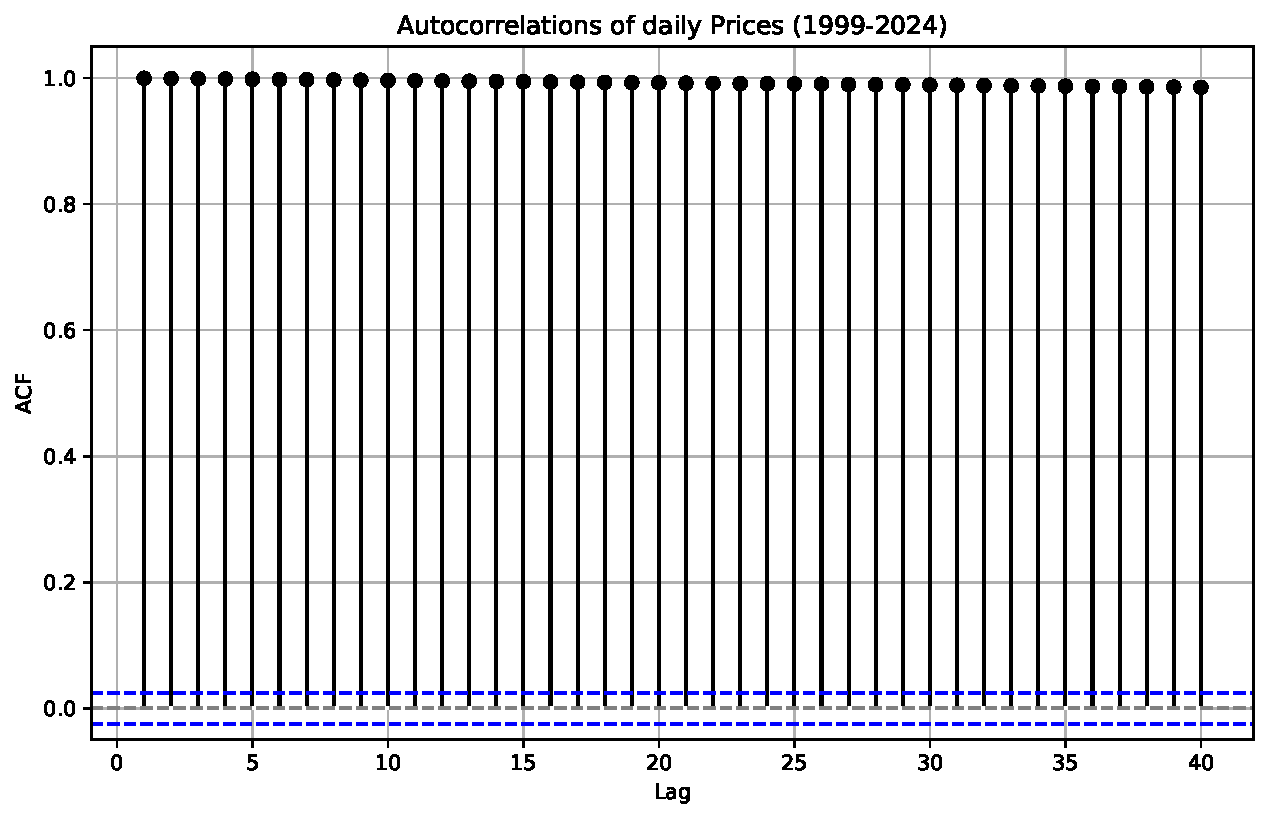
\includegraphics[width=0.8\textwidth]{Img/Autocorrelation.pdf}
    \caption{Autocorrelations of daily Prices (1999-2024)}
    \label{fig:Autocorrelations of daily Prices (1999-2024)}
\end{figure}

\subsection{Returns are stationary}

\appendix

\lstset{
    language=Python,
    backgroundcolor=\color{codebackground},   % Background color
    basicstyle=\ttfamily\footnotesize,        % Font and size
    breaklines=true,                          % Automatic line breaking
    frame=single,                             % Frame around code
    numbers=left,                             % Line numbers on the left
    numberstyle=\tiny\color{gray},            % Line number style
    keywordstyle=\color{codeblue}\bfseries,   % Keyword color
    commentstyle=\color{codegreen}\itshape,   % Comment color
    stringstyle=\color{codepurple},           % String color
    showstringspaces=false,                   % Hide string spaces
    captionpos=b,                             % Caption position: bottom
    tabsize=4                                 % Tab width
}

\section{Appendix: Python Code}
Below is the Python code used in the analysis.

\begin{lstlisting}[caption=Python Code for Analysis]
# Python code example
import numpy as np
import pandas as pd

def analyze_data(data):
    mean = np.mean(data)
    std_dev = np.std(data)
    return mean, std_dev

data = [1, 2, 3, 4, 5]
mean, std_dev = analyze_data(data)
print(f"Mean: {mean}, Standard Deviation: {std_dev}")
\end{lstlisting}
  % Include the code appendix


\end{document}